\section{Геометрические свойства модели Изинга с точки зрения числа соседей в узлах}

\subsection{Сравнение модели Изинга и полимерной цепочки в решетках с 2-6 возможными соседями у мономеров}

\begin{figure}
    \centering
    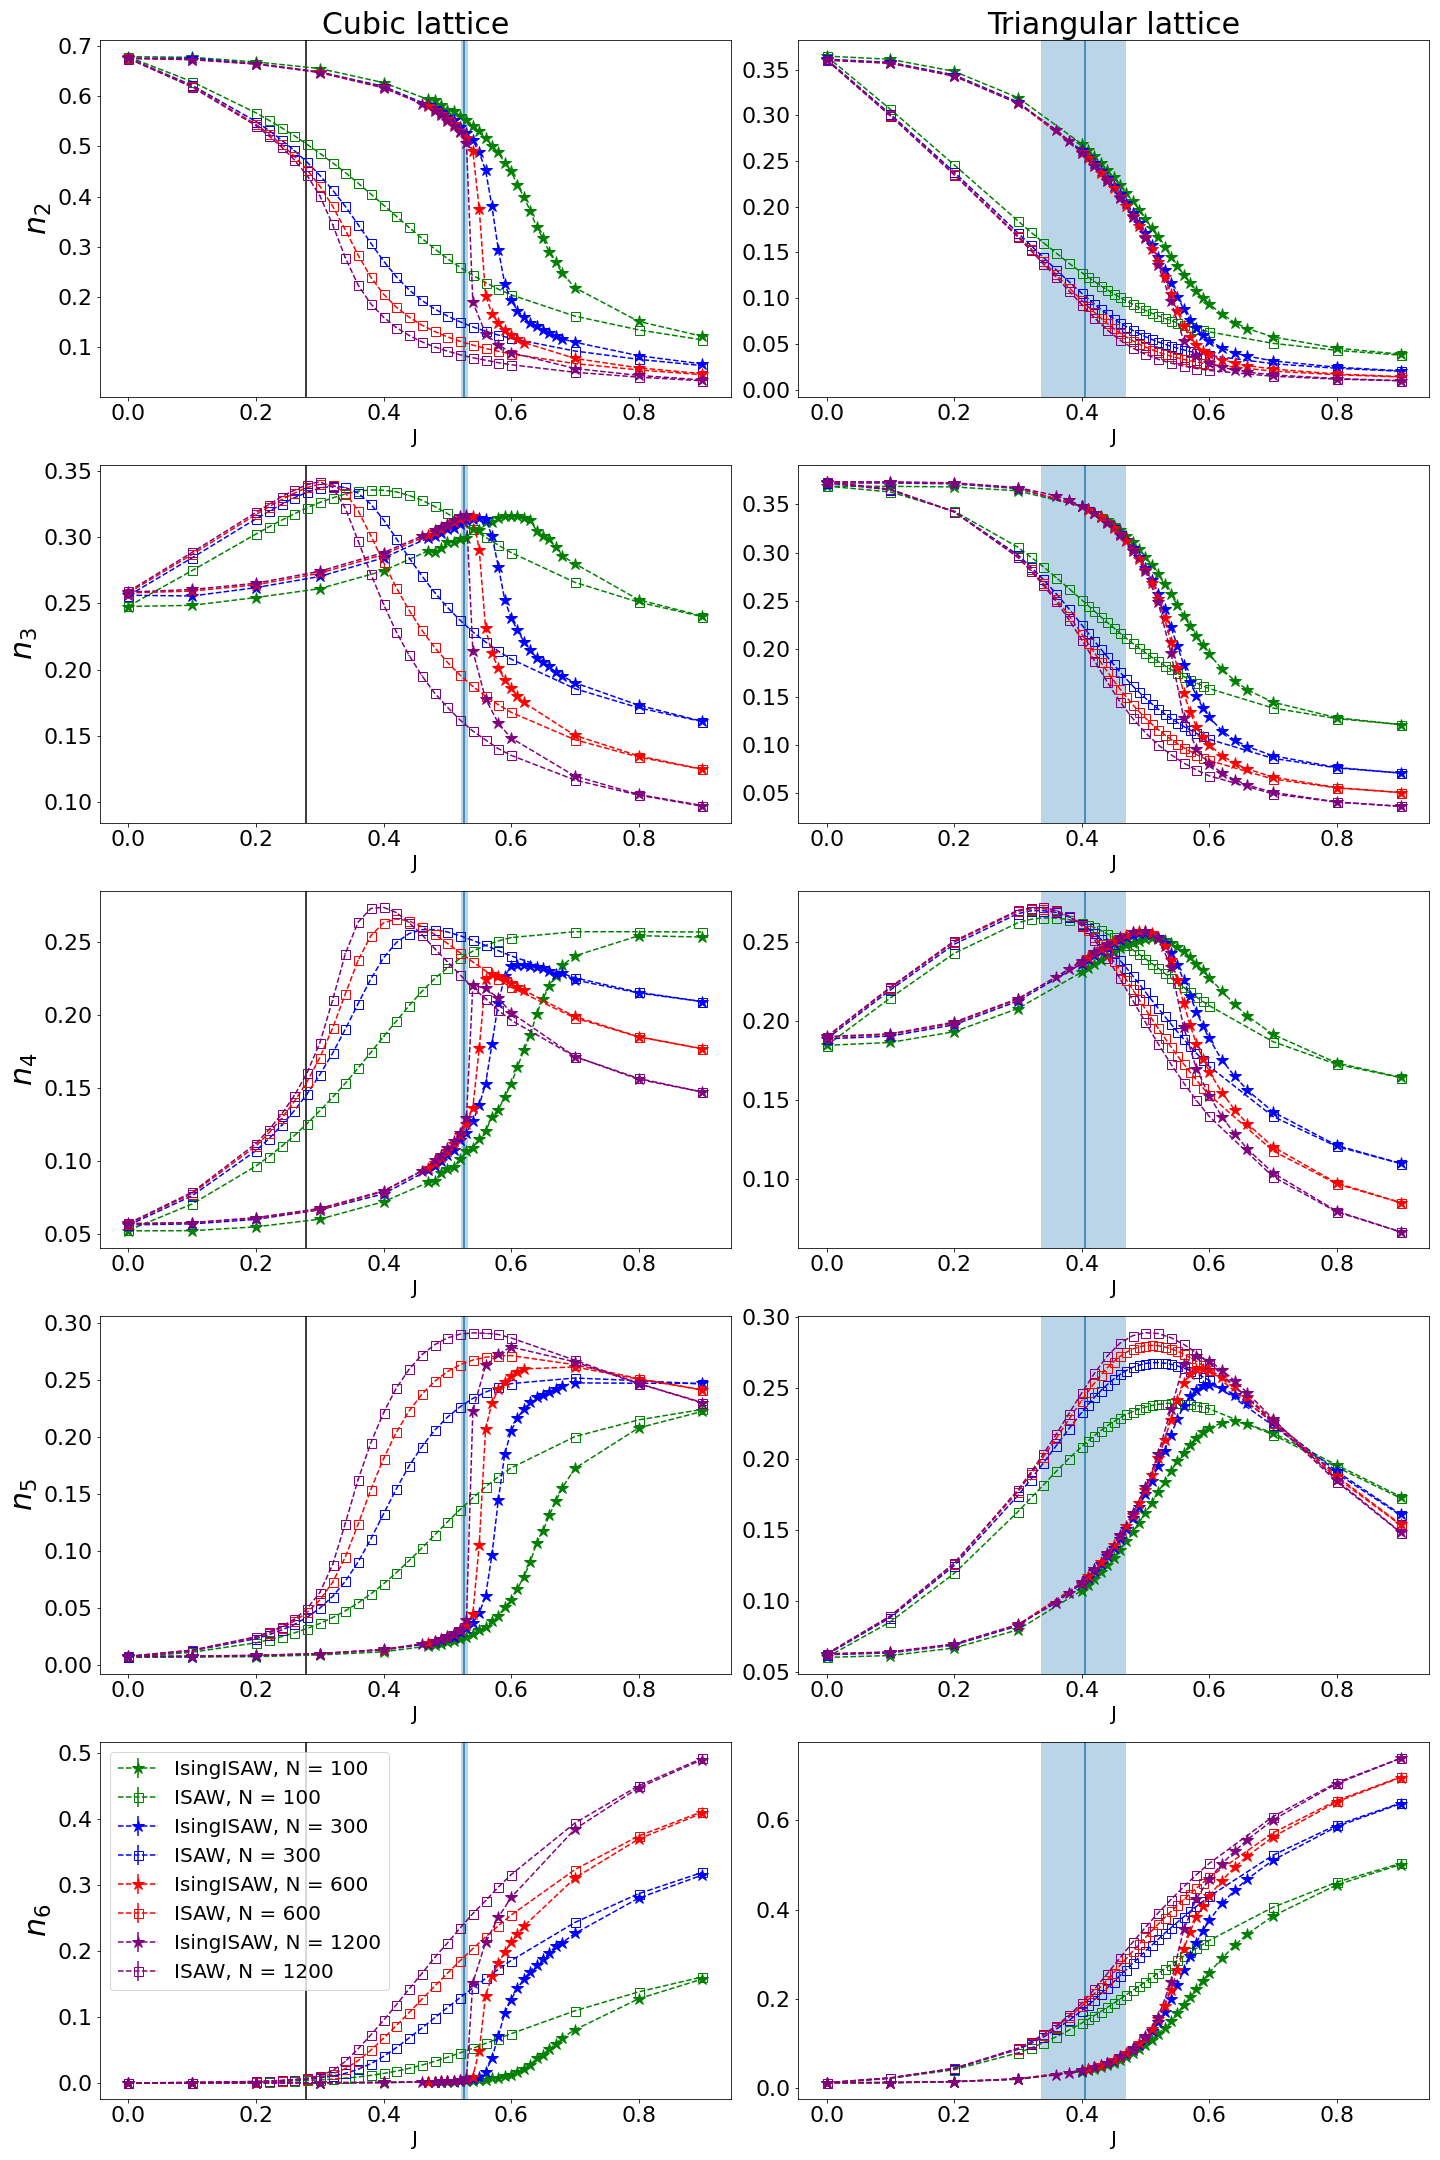
\includegraphics[width=0.95\textwidth, height=21.5cm]{Sections/Images/Ising_vs_ISAW.png}
    \caption{Fractions of monomers of Ising-ISAW model (stars) and ISAW model (open squares) on a cubic lattice (left column) and 2D-triangle lattice (right column) with 2-6 nearest neighbors as function of $J$ with length of conformations $N = $ 100 (green), 300 (blue) and 600 (red). Vertical lines define points of $\theta$-transition (For cubic lattice: black line for ISAW model \cite{Tesi1996} and blue line for Ising-ISAW model \cite{Foster2021}; for triangle lattice: blue line for ISAW model \cite{Privman1986})}
    \label{fig:Ising_vs_ISAW}
\end{figure}

\newpage

\subsection{Сравнение геометрических свойств модели Изинга на треугольной решётке с квадратной}

\begin{figure}
    \centering
    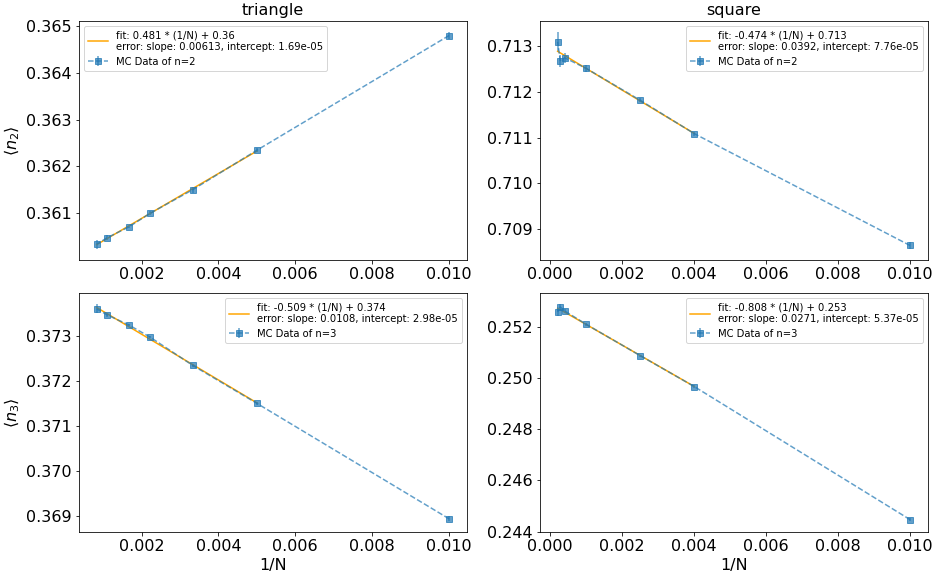
\includegraphics[width=0.95\textwidth]{Sections/Images/triagle_vs_square_bulk.png}
    \caption{Графики зависимости средней доли узлов с 2-3-мя соседями (сверху вниз) от обратной длины 1/N в модели Изинга на треугольной (слева) при N от 200 до 1200 и квадратной (справа) решётках при N от 250 до 4900 при J=0. Синяя линия описывает результаты симуляций Монте-Карло, оранжевая - линейное приближение результатов, ошибки рассчитаны с учётом погрешностей полученных данных}
    \label{fig:tr_vs_sq_bulk}
\end{figure}

На графике \ref{fig:tr_vs_sq_bulk} наглядно показано сравнение приближений долей "одномерных" участков (то есть, долей мономеров с двумя соседями) и узлов с тремя соседями в цепочках на треугольной и квадратной решётках. Для расчётов долей на треугольной решётке были использованы длины 200-1200, для квадратной - 250-4900. Приближение долей треугольной решётки имеет отчётливый линейный характер, включая даже в приближении на всех точках (см. раздел "Подсчёт соседей у треугольной решётки" в Bulk2-6.ipynb\cite{Git}). Линейность долей квадратной решётки также подтверждается (с учётом погрешности расчётов с наибольшей длиной).

Так же хочется заметить некоторое сходство значений свободного члена для долей с двумя соседями и свободного члена в приближениях графика зависимости вероятности гомополимерной цепочки иметь атмосферу 3 в статье Преллберга\cite{Prellberg}, то есть вероятность, что второй конец цепочки длины N имеет 3 возможных направления для удлинения и следовательно, 3 узла, которые могут стать N+1-ым в цепочке.

\begin{table}[]
    \centering
    \begin{tabular}{|c|c|c|c|}
    \hline
    k & $p^{(k)}$ & i & $intercept(\la n_{i} \ra)$ \\ \hline
    3 & 0.711 14(3) & 2 & $0.71299 \pm 2*10^{-5}$ \\ \hline
    2 & 0.225 00(2) & 3 & $0.25291 \pm 10^{-5}$ \\ \hline
    1 & 0.054 76(1) & 4 & $0.03410 \pm 10^{-5}$\\ \hline
    0 & 0.009 096(4) & - & - \\ \hline
    \end{tabular}
    \caption{Таблица сравнения свободных членов линейных приближений вероятностей у конформации иметь n-ю атмосферу (слева) и долей мономеров с i соседями (справа) в зависимости от обратной длины конформации 1/N}
    \label{tab:Prellb_Compare}
\end{table}

На таблице \ref{tab:Prellb_Compare} слева изображены значения свободных членов графика зависимости вероятности гомополимерной цепочки иметь атмосферу k в статье Преллберга\cite{Prellberg}, то есть вероятность, что второй конец цепочки бесконечно большой длины N имеет k возможных направления для удлинения и следовательно, k возможных узлов, которые могут стать новым узлом в цепочке. Справа изображены значения свободных членов приближений графиков долей узлов с i соседями. Хотя все значения отличаются больше чем на погрешность расчётов, однако нельзя не заметить довольно близкое сходство $p^{(3)}$ и свободного члена $\la n_{2} \ra$, хотя сами приближения имеют противоположные по знаку наклоны. 
Возможно, обе величины по-разному описывают одно и то же поведение цепочек с точки зрения их плотности: например, если конец цепочки длины N (назовём его "N-ым узлом") имеет атмосферу три, то при добавлении нового N+1-го узла N-й будет иметь два соседа: N-1-й и N+1-й узлы. Так же при атмосфере 2 (то есть, уже имея два соседа и две возможности для удлинения) N-ый узел при удлинении будет иметь 3 соседа. И наконец, при атмосфере 1 удлинение цепочки приведёт к тому, что старый конец цепочки будет иметь 4 соседа. Очевидно, что случай удлинения при атмосфере 0 рассмореть невозможно, и провести аналогию с соседями нельзя.

Однако сходства между одномерием треугольной и квадратной решётки с точки зрения самих приближений почти не наблюдается - они имеют как разные значения свободных членов, так и значения и даже (в случае 2-х соседей) знаки коэффициента наклона, разница который значительно превышает погрешность фита.



\subsection{Сравнение геометрических свойств модели Изинга на треугольной решётке с кубической}

\begin{figure}
    \centering
    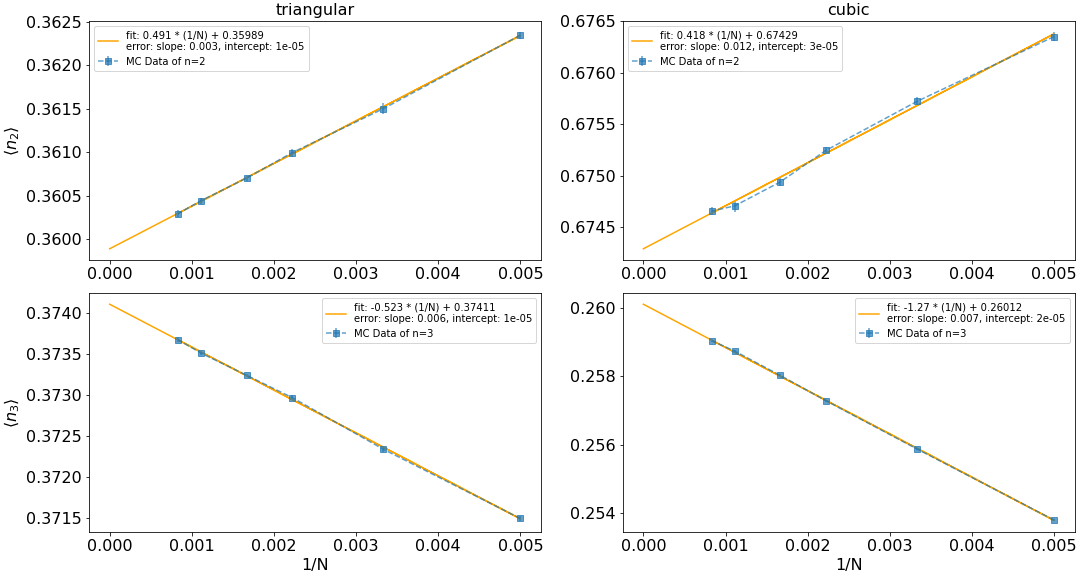
\includegraphics[width=0.95\textwidth]{Sections/Images/triangle_vs_cubic_bulk.png}
    \caption{Зависимость средней доли узлов с 2-3-мя соседями (сверху вниз) от обратной длины 1/N в модели Изинга на треугольной (слева) и кубической (справа) решётках при J=0. Синяя линия описывает результаты симуляций Монте-Карло, оранжевая - линейное приближение результатов, ошибки рассчитаны с учётом погрешностей полученных данных}
    \label{fig:tr_vs_cb_bulk}
\end{figure}

Здесь мы сравниваем линейное приближение треугольной решётки с кубической, имеющейтакое же количество возможных соседей. Получается примерно та же ситуация как и в случае сравнения с квадратной - кубическая решётка на графике \ref{fig:tr_vs_cb_bulk} показывает почти чёткий линейный характер приближения в пределах погрешности наибольших длин (для n=3 линейно видна значительно лучше), но значения не имеют никакого сходства. Единственное отличие от сравнения с квадратной решёткой - графики соответствующих долей имеют одинаковое поведение с точки зрения знака наклона, что действительно и для долей узлов с больший числом соседей. Можно утверждать, что треугольная решётка с точки зрения поведения доли одномерных участок больше похожа на кубическую решётку, нежели квадратную, однако универсальность поведения доли "одномерных" участков среди решёток при бесконечно больших длинах конформации не обнаружена.